\documentclass[conference]{IEEEtran}
\usepackage{balance}
\usepackage{moreverb}
\usepackage{amsmath}
\usepackage[utf8]{inputenc}
\usepackage{pifont}
\usepackage{listings}  
\usepackage{color}  
\usepackage{textcomp}  
\usepackage{url}  

\definecolor{listinggray}{gray}{0.98}  
\definecolor{lbcolor}{rgb}{0.98,0.98,0.98}  
\lstset{  
 backgroundcolor=\color{lbcolor},  
 tabsize=4,  
 rulecolor=,  
 language=java,  
        basicstyle=\scriptsize,  
        upquote=true,  
        aboveskip={1.5\baselineskip},  
        columns=fixed,  
        showstringspaces=false,  
        extendedchars=true,  
        breaklines=true,  
        showtabs=false,  
        showspaces=false,  
        showstringspaces=false,  
        identifierstyle=\ttfamily,  
        keywordstyle=\color[rgb]{0,0,1},  
        commentstyle=\color[rgb]{0.133,0.545,0.133},  
        stringstyle=\color[rgb]{0.627,0.126,0.941},  
}

\ifCLASSINFOpdf
   \usepackage[pdftex]{graphicx}
\else
\fi


\addtolength{\textwidth}{2mm}
\hyphenation{op-tical net-works semi-conduc-tor}

\begin{document}
\title{Data Synchronization and Replication Tool}

\author{\IEEEauthorblockN{Pradeeban Kathiravelu}
\IEEEauthorblockA{INESC-ID Lisboa\\
Instituto Superior T\'{e}cnico, Universidade de Lisboa\\
Lisbon, Portugal\\
Email: pradeeban.kathiravelu@tecnico.ulisboa.pt}
\and
\IEEEauthorblockN{Ashish Sharma}
\IEEEauthorblockA{Department of Biomedical Informatics\\
Emory University\\
Atlanta, Georgia, USA\\
Email: ashish.sharma@emory.edu}}
\maketitle

\begin{abstract}
Consumers download the data by searching the image repository using the browser. The information that the consumer is interested in, gets updated whenever the data producers update or add patient information. The current download tool lacks the ability to track the relevant updates to the consumer. A data replication and synchronization tool will assist automated downloads to the consumers. Users can create replica sets as a sub set of their search queries, and share their replica sets with other users, and update their replica sets periodically. Replica sets can be used as a way of tracking and sharing information. This project exploits this model to create a data replication and synchronization tool for data sources. As a proof of concept, a data replication and synchronization tool has been implemented for The Cancer Imaging Archive (TCIA).
\end{abstract}

\IEEEpeerreviewmaketitle

\section{Introduction}
Data sources contain data of different granularity. Data is organized in a hierarchical structure, where different levels are used to present data in specific formats. Folders and documents make a good example of this. A unique identifier is assigned to each of the data units. A search across the data source would present the user with the list of matching criteria. Interesting sub set of the matching criteria may be bookmarked by the user and shared with others. 

The sub set which is commonly known as a replica set, can be updated, duplicated, shared with other users, and deleted later. A search query may contain different parameters that can define the scope of the search and the outcomes, and often return the outputs in a finer granularity. When a sub set of such information is stored as a replica set, it is sufficient to store the unique identifiers of the matching data units of finer granularity than the original search query, as it would be sufficient to reproduce the data that is represented by the replica set.

\section{Background}
\balance
\subsection{Representation of Medical Images in TCIA}
Medical images are represented in multiple granularity. Figure~\ref{fig:granularity} represents how the images are structured hierarchically in TCIA.
\begin{figure}[b]
\begin{center}
 \resizebox{\columnwidth}{!}{
  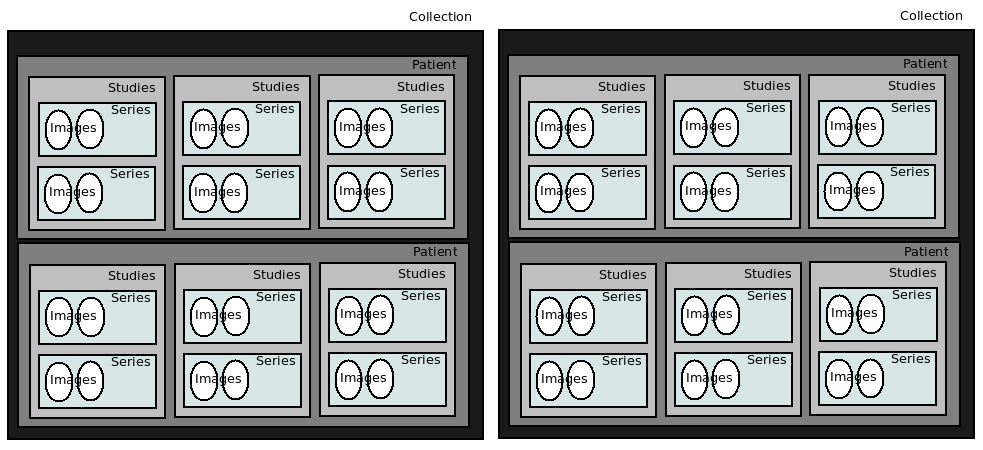
\includegraphics[width=\textwidth]{tcia.png}
 }
\end{center}
 \caption{Medical Images Granularity}
 \label{fig:granularity}
\end{figure}

\section{Design and Implementation}
\balance
Having multiple instances running over different nodes provide fault-tolerance, as when one node terminates, the other nodes have the backup replica of the partitions stored in the terminated node. Figure~\ref{fig:deployment} shows the higher level deployment view of the solution.
\begin{figure}[!htbp]
\begin{center}
 \resizebox{0.6\columnwidth}{!}{
  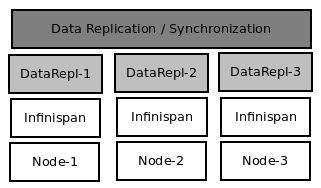
\includegraphics[width=0.6\textwidth]{deployment.png}
 }
\end{center}
 \caption{Deployment}
 \label{fig:deployment}
\end{figure}

\subsection{Generic Design}
Two distributed cache instances exist in InfDataAccessIntegration.
\begin{lstlisting}  
    protected static Cache userReplicasMap;
    protected static Cache replicaSetsMap;
\end{lstlisting}  
userReplicasMap is a mapping of userId \ding{213} Array of replicaSetIDs. UserID could be the logged in user name. (for now, testing with random strings).
replicaSetsMap is a mapping of replicaSetID \ding{213} replicaSet.

Though this could be replaced with a single cache instance with the mapping of userID \ding{213} replicaSets, having two cache instances will be more efficient during searches, duplicates, and push changes. Hence, two cache instances design was chosen.

$InfDataAccessIntegration$ implements the PubConsAPI for publisher/consumer, where $InterfaceManager$ implements the $InterfaceAPI$ for the interface between the data source and the data replication and synchronization tool. Invoker classes extending the abstract class InterfaceManager, implement the respective data source integration to invoke these methods. The execution flow is depicted by Figure~\ref{fig:execution}. When the user logs in, $logIn()$ checks whether the user has already stored replicaSets from the Infinispan distributed Cache. If so, execute them all again. This would be changed later as we do not have to execute all. Rather, we need to execute for the diffs. When the user performs new searches, for the images, series, collections, and the other meta data, the results will be returned to the user, and the user can chose ta subset of the returned results to create a replicaSet.
\begin{figure}[!htbp]
\begin{center}
 \resizebox{\columnwidth}{!}{
  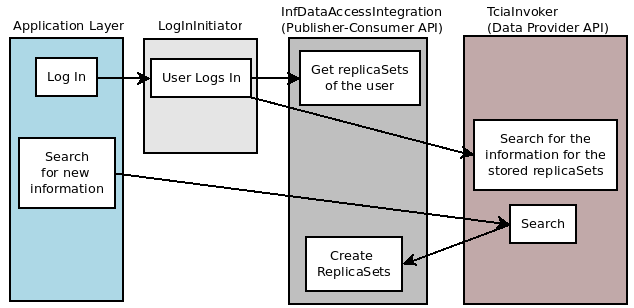
\includegraphics[width=\textwidth]{execFlow.png}
 }
\end{center}
 \caption{Execution Flow}
 \label{fig:execution}
\end{figure}
The replicaSet for the image will be as,
\begin{lstlisting}  
TCIAConstants.IMAGE_TAG + "getImage?SeriesInstanceUID=" + seriesInstanceUID
\end{lstlisting}  
For other information (meta data), such as collections and seies,
\begin{lstlisting}  
TCIAConstants.META_TAG + query;
\end{lstlisting}  

Here, query takes the below format. 
\begin{lstlisting}  
"getSeries?format=" + format +
                "&Collection=" + collection +
                "&PatientID=" + patientID +
                "&StudyInstanceUID=" + studyInstanceUID +
                "&Modality=" + modality;
\end{lstlisting}  
When a new instance starts now, and invokes the log in action for the same user, it will execute the queries for the stored replicaSets again, and reproduce the same results.

\subsection{Design and Implementation for TCIA}
Different complex data sources require custom development extending the generic framework. As creating and customizing the replicaSet require a more specific data structure, further implementations are done, extending the core class hierarchy. An extension based on the base design was developed for TCIA, as shown by Figure~\ref{fig:class}, which provides a core class hierarchy of the system.
\begin{figure}[b]
\begin{center}
 \resizebox{0.8\columnwidth}{!}{
  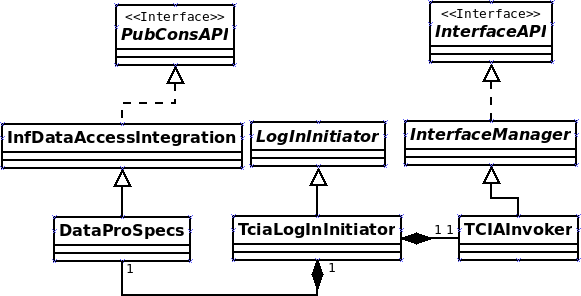
\includegraphics[width=0.8\textwidth]{classDiagram.png}
 }
\end{center}
 \caption{Core Class Hierarchy}
 \label{fig:class}
\end{figure}

$TciaInvoker$ extends $InterfaceManager$ to implement the interfacing layer between the TCIA data source and the data replication and synchronization tool. Meta data such as collections, patients, studies, and series are retrieved at different levels, though the default download manager of TCIA downloads the data in series level, composed of the images of the series in a single zip archive. While having the default userReplicasMap to contain the IDs of the replica sets for each user, the replica set itself is stored in multiple maps instead of a single replicaSets map, to provide an efficient storage and access.

$DataProSpecs$ extends the $InfDataAccessIntegration$ class. 5 maps are created as below to represent the replica sets.
\begin{lstlisting}  
    protected static Cache<Long, Boolean[]> tciaMetaMap;
    protected static Cache<Long, String[]> collectionsMap;
    protected static Cache<Long, String[]> patientsMap;
    protected static Cache<Long, String[]> studiesMap;
    protected static Cache<Long, String[]> seriesMap;
\end{lstlisting} 

$tciaMetaMap$ contains a boolean array, which reflects which of the granularity of meta data is selected as a whole. For TCIA, if a few collections are selected, the first element of the array is set to true, and similarly, the other meta data are marked to true or false as shown by the below code segment.
\begin{lstlisting}  
        Boolean[] metaMap = new Boolean[4];
        metaMap[0] = collection != null;
        metaMap[1] = patientID != null;
        metaMap[2] = studyInstanceUID != null;
        metaMap[3] = seriesInstanceUID != null;

        putReplicaSet(replicaSetId, metaMap);
\end{lstlisting} 
The name of the collections, patientID, studyInstanceUID, and seriesInstanceUID are stored against the respective replicaSetID in collectionsMap, patientsMap, studiesMap, and seriesMap respectively. Hence changes are done at the respective maps. Duplicating the replicaSets duplicate the contents of the entire row to a new replicaSetID. Similarly, deleting a replicaSet deletes the respective information from all the maps.

TCIA public API provides methods to retrieve the images and meta data of different granularity. Figure~\ref{fig:methods} depict the methods that retrieve image and metadata at different granularity from TCIA. These methods are invoked by the replication manager tool to retrieve the images. As shown by Figure~\ref{fig:methods} an initial search on TCIA may contain parameters such as modality, in addition to collection name, patient ID, study instance ID, and series instance UID. However, each of these search returns the output in a finer granularity, and when a sub set of this finer granularity is selected, each of the selected elements are always identified by their respective identifier. Hence, storing an array of patient ID would be sufficient to identify the selected sub set of the collection including the array of patients. Similary an array of study instance UID is sufficient to represent the selected sub set of any patient, and an array of series instance UID is sufficient to represent the selected sub set of any study, as it will contain an array of series.

\begin{figure}[!htbp]
\begin{center}
 \resizebox{\columnwidth}{!}{
  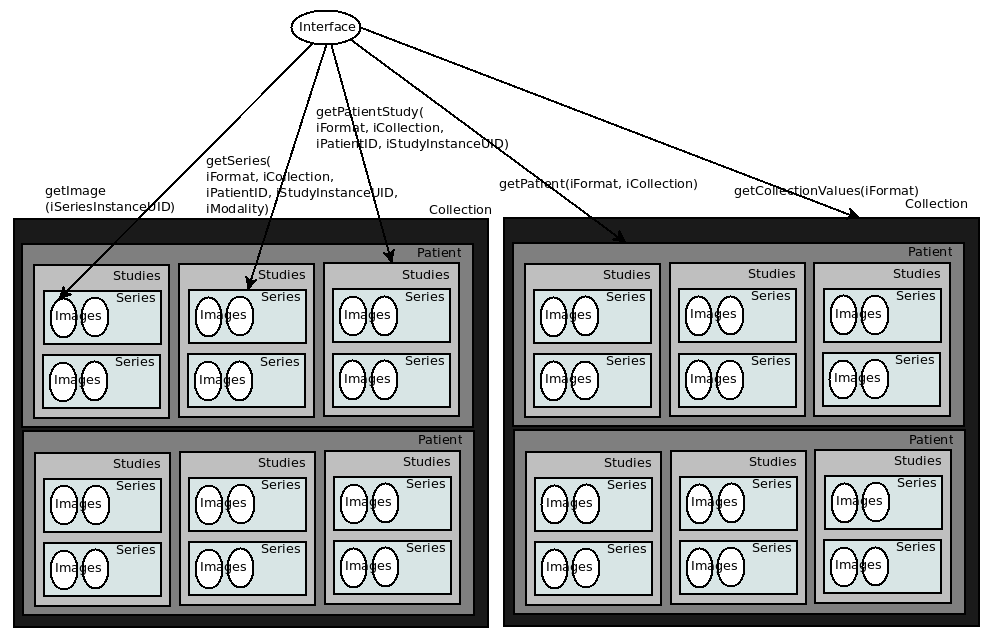
\includegraphics[width=\textwidth]{methods.png}
 }
\end{center}
 \caption{Retrieving images and meta data}
 \label{fig:methods}
\end{figure}

\paragraph*{Prototype Web Application Development}
A prototype web application is built with the data replication and synchronization tool and TCIA REST API. Apache Velocity is used to generate the web pages for the replication tool. Apache Tomcat (Embedded) is integrated into the program such that it will get the user inputs from the HTML pages and present the output in pages formatted by Apache Velocity Templates. Respective servlets are created inside the servlets package to receive the inputs from HTML pages to the backend Java code.

$DataRetriever$ class is invoked to retrieve the meta data from TCIA and to create and retrieve replica sets. $UIGenerator$ class invokes the Apache Velocity templates to create the web pages, presenting the data to the users. $DataRetriever$ has instances of $TciaInvoker$ and $TciaLogInInitiator$ to invoke the TCIA queries and replication tool create and retrieve replicaSets mechanisms. $TciaLogInInitiator$ has instances of $TciaInvoker$ and $DataProSpecs$, to invoke the public APIs provided by these classes for the data provider specification and publisher/consumer APIs. Figure~\ref{fig:classUX} depicts the class hierarchy involved in the user interface.
\begin{figure}[!htbp]
\begin{center}
 \resizebox{0.45\columnwidth}{!}{
  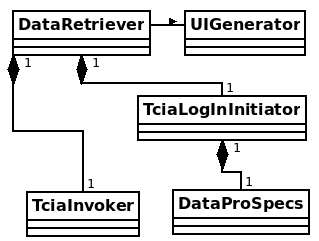
\includegraphics[width=0.45\textwidth]{classUX.png}
 }
\end{center}
 \caption{Class Hierarchy of the User Interface}
 \label{fig:classUX}
\end{figure}


\paragraph*{multi-tenancy}
The Replication Tool is multi-tenanted, and it is aware of the multiple tenants or users using the system. The methods of $DataProSpecs$ can be invoked by knowing the respective replicaSetID of the replica set and the user ID of the user who owns the replica set. User ID is a random string that is input by the user. Probably this can be some 'secret' or pass from the user. userIDs serve as the keys of the userReplicasMap. Apart from that, there is no data structure to hold the list of users.

$createReplicaSet()$ requires the userID along with the elements to be stored in the replica set. It returns the $replicaSetID$, which is further used to uniquely identify the replica set. $getReplicaSet()$ requires only the relevant $replicaSetID$ to return the respective replica set. Similarly, $updateReplicaSet()$ requires $replicaSetID$ as well as the elements to be stored in the $replicaSet$, replacing the previous elements. $deleteReplicaSet()$ requires both the $userID$ and $replicaSetID$. Similarly, $duplicateReplicaSet()$ requires both $replicaSetID$ and the userID of the user to whom the replicaSet is shared to. Creating, deleting, and duplicating a replication set requires modification to the user replicas map, which holds the list of the replica sets for the particular user. Hence the necessity to input the userID. ReplicaSetID is a large negative number (UUID) randomly generated. It can be safely assumed to be harder to guess. Hence, this model is assumed to provide adequate security for this prototype.


\section{Evaluation}
\section{Conclusion}
Storing a selected sub set of data items that matches a specific criteria as a replica set is an optimal way to bookmark large data sources. Users should be able to create and update their replica sets, and share it with others using a unique identifier. While different data sources have different interfaces, a generic data replication and synchronization tool will be convenient, such that sharing of replica sets across heterogeneous data sources will be possible. This project researched the possibilities of such a replication and data synchronization tool, exploiting the in-memory data grid projects, and implements a data synchronization and replication tool\footnote{The source code can be accessed from \url{https://bitbucket.org/BMI/datareplicationsystem}} with Infinispan while consuming data sources such as TCIA via their public APIs.


%\begin{thebibliography}{1}
%\end{thebibliography}

\end{document}


